\documentclass[14pt]{beamer}
\usetheme{default}
\usepackage[L7x,T1]{fontenc}
\usepackage[lithuanian]{babel}
\usepackage{graphics}
\usepackage{biblatex}
\usepackage{tabularx}
\usepackage[labelfont={color=vupurple},labelformat=empty,justification=centering]{caption}
\usepackage{tikz}
\usepackage{minted}
\usepackage{subcaption}


\definecolor{vulightgrey}{RGB}{220,220,220}
\definecolor{vudarkgrey}{RGB}{65,65,65}
\definecolor{vupurple}{RGB}{123,0,63}
\definecolor{darkgreen}{RGB}{32,96,32}
\setbeamercolor{title}{fg=vupurple}
\setbeamercolor{frametitle}{fg=vupurple}
\setbeamercolor{abstract title}{fg=vupurple}
\setbeamercolor{item}{fg=vupurple}
\setbeamercolor{navigation symbols dimmed}{fg=vulightgrey}
\setbeamercolor{navigation symbols}{fg=vulightgrey}
\setbeamercolor{normal text}{fg=vudarkgrey}

\usefonttheme{serif}

\AtBeginEnvironment{minted}{%
    \renewcommand{\fcolorbox}[4][]{#4}}
\usetikzlibrary{shapes.geometric,arrows,positioning}

\newcommand{\DP}{Douglas \& Peucker}
\newcommand{\VW}{Visvalingam--Whyatt}
\newcommand{\WM}{Wang--M{\"u}ller}

\mode<presentation>{
    \setbeamertemplate{navigation symbols}{
        \insertslidenavigationsymbol
        \insertframenavigationsymbol
        \hspace{0.2cm}
        \begin{minipage}[c]{0.5cm}
            \vspace{-0.1cm}
            {\strut\insertframenumber{}/\inserttotalframenumber\strut}
        \end{minipage}
    }
}

\newcommand{\twocols}[2]
{
    \begin{columns}[c]
        \begin{column}{0.45\textwidth}
            #1
        \end{column}
        %\hspace{0pt} \vrule{}
        \begin{column}{0.55\textwidth}
            #2
        \end{column}
    \end{columns}
}

%% =============================================================================

\title{
    \Large\textsc{wang–müller algoritmo realizacija 
    kartografinei upių generalizacijai}

}
\author{\small \bf Motiejus Jakštys \\[4ex]
    
\includegraphics[height=4em]{vu}
}

\date{\small 2021-06-02}


\begin{document}


\AtBeginSection[]
{
  \begin{frame}
    \frametitle{Turinys}
    \tableofcontents[currentsection]
  \end{frame}
}

\begin{frame}
\titlepage
\end{frame}

\begin{frame}
  \begin{abstract}

    Dabartiniai linijų simplifikavimo algoritmai netinka upėms. Šis darbas
    realizuoja {\WM} algoritmą. Jis geriau tinka upėms.

  \end{abstract}
\end{frame}

\section{Problema}

\begin{frame}{Linijų paprastinimo algoritmų problemos}
  \twocols{
    \begin{figure}[ht]
      \includegraphics[width=\textwidth]{salvis-dp64-2x50k}
      \caption{\footnotesize Paprastinta naudojant {\DP}.}
    \end{figure}
  }{
    \begin{itemize}
      \item Nepritaikyti gamtiniams objektams: upėms, krantų linijoms.
      \item Prarandami raiškūs gamtinių objektų elementai: vingiai, kilpos.
    \end{itemize}
  }
\end{frame}

\section{Uždaviniai}

\begin{frame}{Uždaviniai: algoritmų vertinimas}
  \twocols{
    \begin{figure}[ht]
      \includegraphics[width=\textwidth]{salvis-overlaid-vwchaikin64-2x50k}
      \caption{\footnotesize GRPK10 ir {\VW}+Chaikin}
    \end{figure}
  }{
    \begin{itemize}
      \item Įvertinti prieinamus linijų paprastinimo algoritmus.
      \item Įvardinti prieinamų algoritmų problemas.
    \end{itemize}
  }
\end{frame}


\begin{frame}{Uždaviniai: {\WM} realizacija}
  \twocols{
    \begin{figure}[ht]
      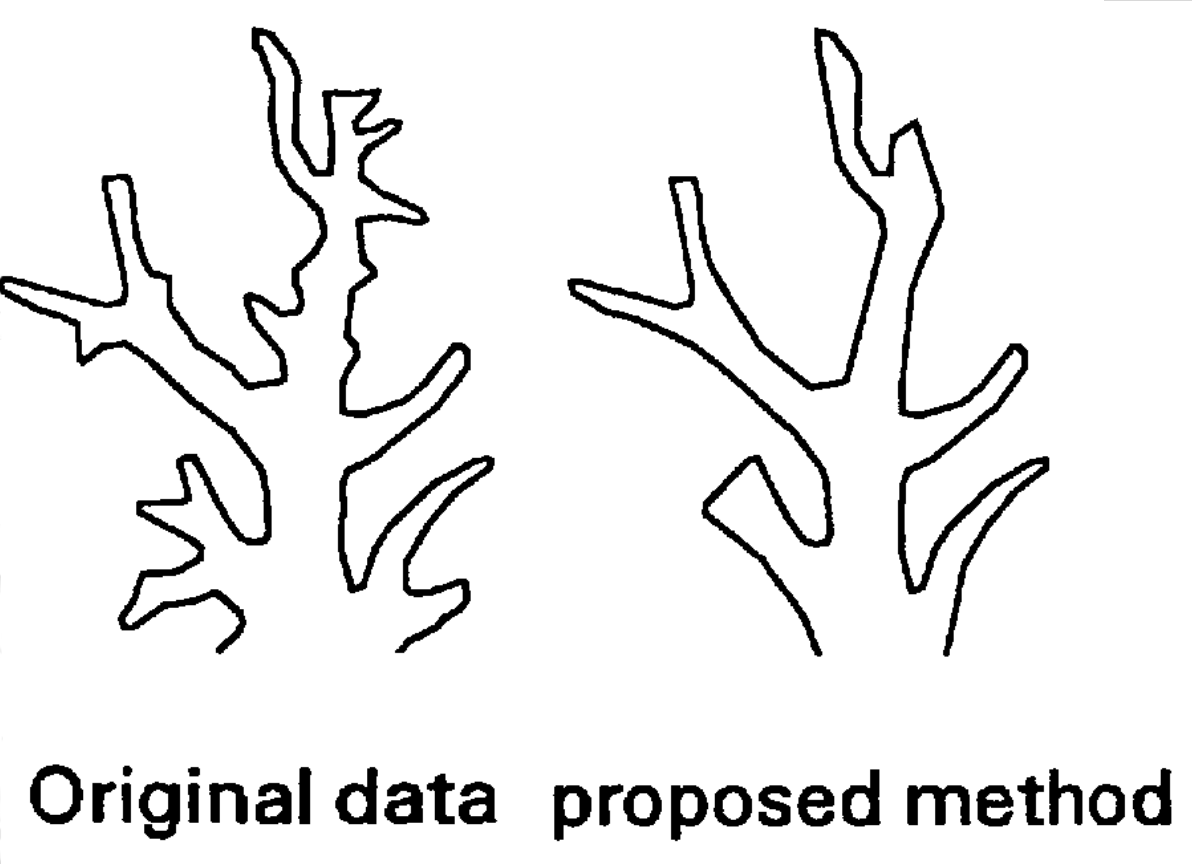
\includegraphics[width=\textwidth]{wang125-2}
      \caption{{\WM} siūlomas metodas.}
    \end{figure}

  }{
    \begin{itemize}
        \item Apibrėžti algoritmo techninės realizacijos metodiką.
        \item Teoriškai ir techniškai realizuoti algoritmą.
        \item Išbandyti su skirtingais duomenų rinkiniais.
        \item Palyginti su valstybiniais duomenų rinkiniais.
    \end{itemize}
  }
\end{frame}

%      \begin{minted}[fontsize=\tiny]{sql}
%CREATE FUNCTION ST_SimplifyWM(
%  geom geometry,
%  dhalfcircle float,
%) RETURNS geometry AS $$
%  ...
%end $$ language plpgsql;
%      \end{minted}

\section{Aktualumas}

\begin{frame}[fragile]{Aktualumas: praplečiama teorija}
  \begin{columns}[c]
    \begin{column}{.3\textwidth}
      \begin{figure}[ht]
        \includegraphics[width=\textwidth]{selfcrossing-1}
      \end{figure}
    \end{column}
    \begin{column}{.7\textwidth}
      \begin{itemize}

        \item Praplečia išplėsti kartografinės teorijos žinias apie gamtinių
          objektų ribų generalizavimą atsižvelgiant į jų raiškumą.

        \item {\WM} straipsnis sprendimų nedetalizuoja taip, kad būtų
          galima pritaikyti. Šis darbas tai padaro.

      \end{itemize}
    \end{column}
  \end{columns}
\end{frame}

\begin{frame}{Aktualumas: panaudojimas}
  \begin{columns}[c]
    \begin{column}{.3\textwidth}
      \begin{figure}[ht]
        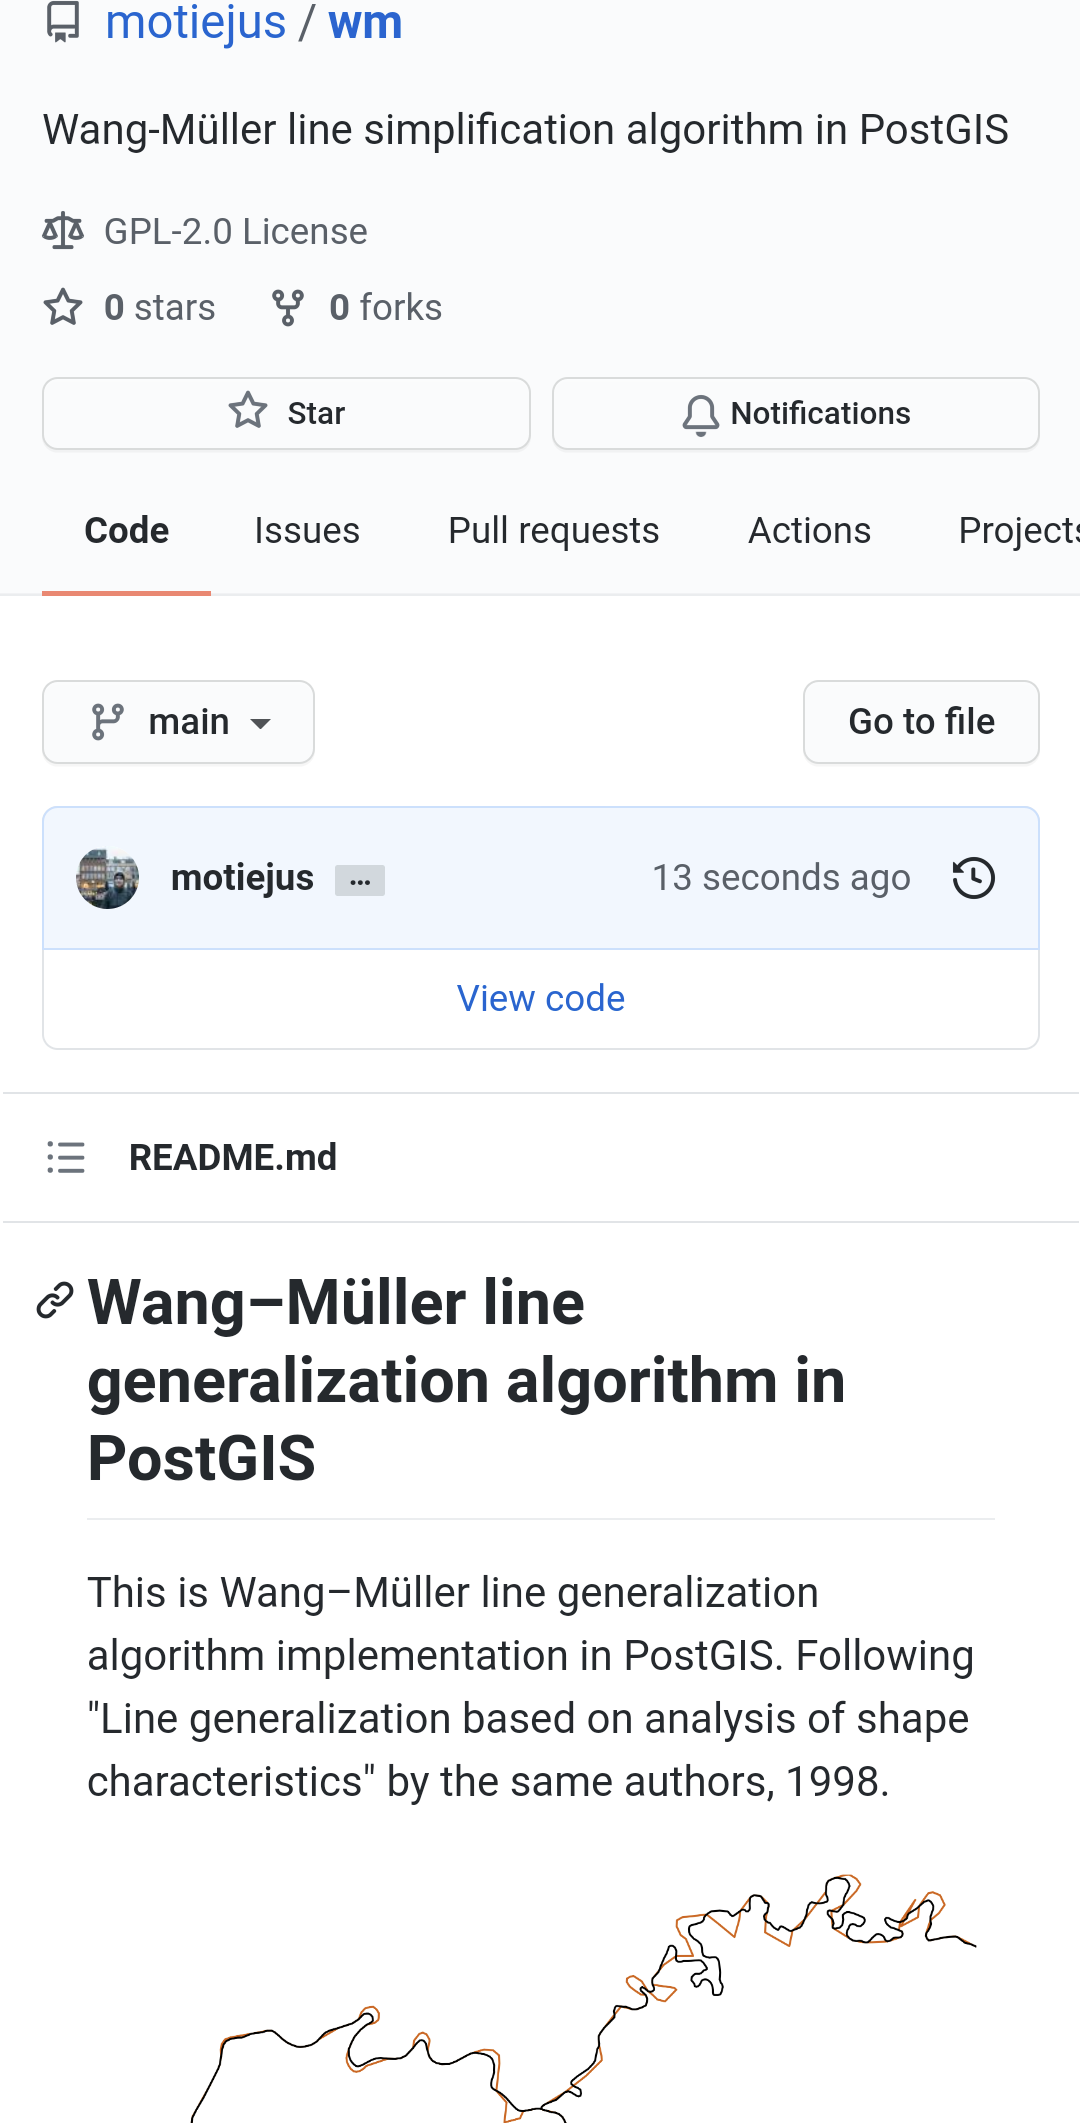
\includegraphics[width=\textwidth]{github-wm}
      \end{figure}
    \end{column}
    \begin{column}{.7\textwidth}
      \begin{itemize}

        \item Papildomas atviro kodo sprendimas automatiniam generalizavimo
          uždaviniams.

        \item Pritaikomas kartografų.

      \end{itemize}
    \end{column}
  \end{columns}
\end{frame}


\section{Metodika}

\begin{frame}{Techninė implementacija: aplinka}
  \begin{columns}[c]
    \begin{column}{.3\textwidth}
      \begin{figure}[ht]
        \begin{subfigure}[b]{\textwidth}
          \centering
          
\includegraphics[width=.7\textwidth]{postgis-logo}
        \end{subfigure}
        \\[1ex]
        \begin{subfigure}[b]{\textwidth}
          \centering
          
\includegraphics[width=.5\textwidth]{postgresql-logo}
        \end{subfigure}
        \\[1ex]
        \begin{subfigure}[b]{\textwidth}
          \centering
          
\includegraphics[width=.6\textwidth]{osi-logo}
        \end{subfigure}
      \end{figure}
    \end{column}
    \begin{column}{.7\textwidth}

      \begin{itemize}
        \item Realizacija kurta PostGIS.

        \item PostGIS yra PostgreSQL duomenų bazės papildinys darbui su GIS.

        \item Atviro kodo nemokama programinė įranga.

        \item PostGIS sprendimai veikia iš praktiškai bet kokios programavimo
          kalbos, todėl yra universalūs.

      \end{itemize}

    \end{column}
  \end{columns}
\end{frame}


\begin{frame}{Techninė implementacija: algoritmas}
    \begin{itemize}[<+->]

        \item Algoritmas implementuotas funkcija \textsc{st\_simplifywm}.

        \item Priima vieną parametrą: \textsc{dhalfcircle}: pusskritulio
            skersmuo: analogiško ir didesnio ploto linkių nepaprastina.

        \item Pagalbinės funkcijos:
            \begin{itemize}
                \item<4> \textsc{wm\_detect\_bends}
                \item<4> \textsc{wm\_fix\_gentle\_inflections}
                \item<4> \textsc{wm\_self\_crossing}
                \item<4> \textsc{wm\_bend\_attrs}
                \item<4> \textsc{wm\_st\_split}
                \item<4> \textsc{wm\_exaggerate\_bend}
                \item<4> ...
            \end{itemize}

    \end{itemize}
\end{frame}

\begin{frame}{Algoritmo realizacijos procesas}
  \tikzset{
    startstop/.style={trapezium,text centered,minimum height=2em,
      trapezium left angle=70,trapezium right angle=110,draw=black,fill=red!20},
    proc/.style={rectangle,minimum height=2em,text centered,draw=black,
      fill=orange!20},
    decision/.style={diamond,minimum height=2em,text centered,aspect=3,
      draw=black,fill=green!20},
    arrow/.style={thick,->,>=stealth},
  }
  \begin{figure}
    \centering
    \scalebox{.35}{
      \begin{tikzpicture}[node distance=2cm,auto]
        \node (start) [startstop] {Nuskaityti \textsc{linestring}};
        \node (detect) [proc,below of=start] {Aptikti linkius};
        \node (inflections) [proc,below of=detect] {Sutvarkyti nežymius išlinkimus};
        \node (selfcrossing) [proc,below of=inflections] {Pašalinti save kertančias vietas};
        \node (mutated1) [decision,below of=selfcrossing] {Koreguotas?};
        \node (bendattrs) [proc,below of=mutated1] {Apskaičiuoti linkio savybes};
        \node (exaggeration) [proc,below of=bendattrs] {Didinti linkį};
        \node (mutated2) [decision,below of=exaggeration] {Koreguotas?};
        \node (elimination) [proc,below of=mutated2] {Pašalinti linkį};
        \node (mutated3) [decision,below of=elimination] {Koreguotas?};
        \node (stop) [startstop,below of=mutated3] {Pabaiga};
    
        \coordinate [right of=mutated1,node distance=5cm] (mutated1y) {};
        \coordinate [right of=mutated2,node distance=5cm] (mutated2y) {};
        \coordinate [right of=mutated3,node distance=5cm] (mutated3y) {};
    
        \draw [arrow] (start) -- (detect);
        \draw [arrow] (detect) -- (inflections);
        \draw [arrow] (inflections) -- (selfcrossing);
        \draw [arrow] (selfcrossing) -- (mutated1);
        \draw [arrow] (mutated1) -| node [near start] {Taip} (mutated1y) |- (detect);
        \draw [arrow] (mutated1) -- node[anchor=west] {Ne} (bendattrs);
        \draw [arrow] (bendattrs) -- (exaggeration);
        \draw [arrow] (exaggeration) -- (mutated2);
        \draw [arrow] (mutated2) -| node [near start] {Taip} (mutated2y) |- (detect);
        \draw [arrow] (mutated2) -- node[anchor=west] {Ne} (elimination);
        \draw [arrow] (mutated3) -| node [near start] {Taip} (mutated3y) |- (detect);
        \draw [arrow] (mutated3) -- node[anchor=west] {Ne} (stop);
        \draw [arrow] (elimination) -- (mutated3);
      \end{tikzpicture}
    }
  \end{figure}
\end{frame}

\begin{frame}{Automatiniai testai padeda tęstinumui}
  \tikzset{
    arrow/.style={thick,->,>=stealth},
  }
  \begin{figure}
    \begin{tikzpicture}[auto]
      \onslide<1->{
        \node (before) []{
          \includegraphics[width=.4\textwidth]{isolated-1-before.pdf}
        };
      }
      \onslide<2->{
        \node(after) [right=2cm of before.east]{
          \includegraphics[width=.4\textwidth]{isolated-1-after.pdf}
        };
      }
      \onslide<2->{
        \draw[arrow] (before) -- node[anchor=south] {\footnotesize Programa} (after);
      }
    \end{tikzpicture}
  \end{figure}
  \onslide<3->{
    \begin{itemize}
      \item<3-> Iš duomenų ir rezultato sukuriamas testas.
      \item<4-> Testai patikrina, ar programa veikia teisingai.
      \item<4-> Išsaugomas tęstinumas ją keičiant.
    \end{itemize}
  }
\end{frame}

\section{Įgyvendinimas}

\begin{frame}{Pasiruošimas}
  \begin{itemize}
    \item Klaidų ieškojimas.
    \item Upių sujungimas.
  \end{itemize}
\end{frame}

\begin{frame}{Algoritmo etapai}
  \begin{itemize}
    \item Linkių aptikimas ir sutvarkymas.
    \item Linkių keitimo operatoriai: eliminavimas ir didinimas.
    \item Jungimas neimplementuotas.
  \end{itemize}
\end{frame}

\section{Rezultatai}

\begin{frame}{GRPK10 ir {\WM}}
  \includegraphics[width=\textwidth]{salvis-wm75--grpk10-1x50k}
\end{frame}

\begin{frame}{GRPK10, GRPK50 ir {\WM}}
  \includegraphics[width=\textwidth]{salvis-wm75-grpk50-grpk10-1x50k}
\end{frame}

\begin{frame}{GRPK250 ir {\WM}}
  \begin{figure}[h!]
    \centering
    \begin{subfigure}[b]{.49\textwidth}
      \includegraphics[width=\textwidth]{salvis-grpk250-2x}
      \caption{GRPK250.}
    \end{subfigure}
    \hfill
    \begin{subfigure}[b]{.49\textwidth}
      \centering
      \includegraphics[width=\textwidth]{salvis-wm220}
      \caption{{\WM}.}
    \end{subfigure}
  \end{figure}
\end{frame}

\begin{frame}{{\DP}}
  \includegraphics[width=\textwidth]{salvis-wm75-dp64-grpk10-1x50k}
\end{frame}

\begin{frame}{{\DP}+Chaikin}
  \includegraphics[width=\textwidth]{salvis-wm75-dpchaikin64-grpk10-1x50k}
\end{frame}

\begin{frame}{{\VW}}
  \includegraphics[width=\textwidth]{salvis-wm75-vw64-grpk10-1x50k}
\end{frame}

\begin{frame}{{\VW}+Chaikin}
  \includegraphics[width=\textwidth]{salvis-wm75-vwchaikin64-grpk10-1x50k}
\end{frame}

\begin{frame}{Išbandymas internete}
  \centering
  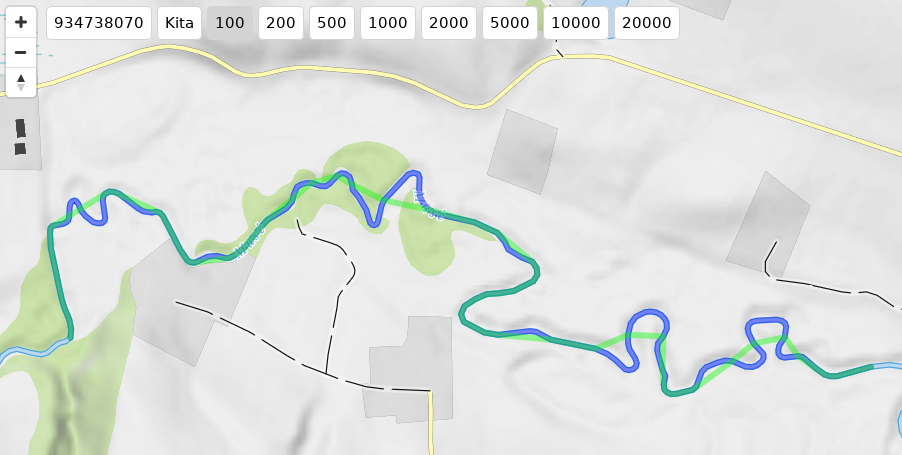
\includegraphics[width=.75\textwidth]{openmap-wm-good.png}
  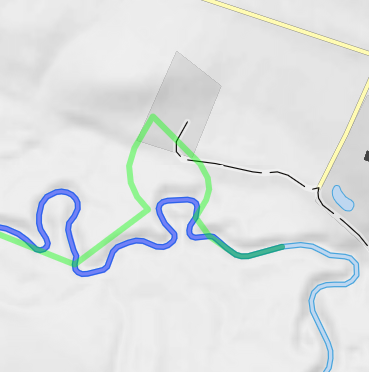
\includegraphics[width=.3\textwidth]{openmap-wm-bad.png}

  {\tiny https://dev.openmap.lt/webgl/wm.html}
\end{frame}

\begin{frame}{Išvados}
  \begin{itemize}
    \item Klasikiniai algoritmai išanalizuoti, problemos aprašytos.
    \item Aprašytas metodas {\WM} realizacijai.

    \item Realizuotas:
      \href{https://github.com/motiejus/wm}{github.com/motiejus/wm}.

    \item Rezultatai palyginti su klasikiniais algoritmais ir GRPK.
  \end{itemize}
\end{frame}

\begin{frame}{Pasiūlymai ateičiai}
  \begin{itemize}
    \item Sukurti kobinavimo operatorių.
    \item Rasti ir aprašyti geresnius kriterijus izoliuotiems linkiams.
    \item Pagerinti algoritmo laiko ir atminties sąnaudas.
    \item Pilnesnė kartografinė generalizacija, įskaitant topologiją.
  \end{itemize}
\end{frame}

\begin{frame}{Ačiū}
  Klausimai? \\ \\

  Techninę realizaciją ir magistrinį darbą rasite
      \href{https://github.com/motiejus/wm}{github.com/motiejus/wm}.
\end{frame}

\end{document}
